\documentclass{beamer}
\mode<presentation>{
	\usetheme{Madrid}
}

\usepackage{graphics}
\usepackage{lipsum}
\usepackage{tikz}
\graphicspath{{./pictures}}
\usepackage[T1]{fontenc}
\usepackage{polski}
\title[]{Analiza porównawcza zastosowań tradycyjnych oraz wariacyjnych autoenkoderów}
\institute[UMCS]
{
	Uniwersytet Marii Curie Skłodowskiej
	\medskip
}
\author{Filip Ręka}
\date{\today}

\begin{document}
% 1
	\begin{frame}
		\titlepage
	\end{frame}

	\begin{frame}
		\tableofcontents
	\end{frame}
% 2
	\begin{frame}
		\frametitle{Cele}
		\section{Cel}
		\begin{itemize}
			\item Analiza możliwości i zastosowań autoenkoderów
			\item Możliwości generacji nowych danych przy użyciu autoenkodera
			\item Charakterystyka architektury autoenkodera wariacyjnego
			\item Analiza możliwości generacji danych przez autoenkoder wariacyjny
			\item Ocena możliwości zastosowania autoenkoderów wariacyjnych do generacji obrazów
		\end{itemize}
	\end{frame}
% 3
	\begin{frame}
		\frametitle{Autoenkoder - wprowadzenie}
		\section{Autoenkoder - wprowadzenie}
		Autoenkoder składa się z dwóch części: enkodera oraz dekodera. Obie z nich są w pełni połączonymi sieciami neuronowymi, które również są połączone pomiędzy sobą. Zadaniem enkodera jest zakodowanie jego wejścia do kodu o stałej długości, co jest osiągane przez architekturę warstw, w której każda następna ma mniej neuronów niż poprzednia. Dekoder jest częścią, która z kodu, próbuje odwzorować zakodowane dane. Cały autoenkoder dostaje na warstwę wejściową oraz wyjściową te same dane, przez co jego sposób uczenia jest nazywany częściowo nadzorowanym. 
	\end{frame}

% 4
	\begin{frame}
		\frametitle{Architektura autoenkodera}
		\begin{figure}
			\centering\includegraphics[width=10cm]{tikzae.pdf}
%			\caption{Przykładowa architektura modelu}
			% + funkcjia aktywacji 
			% nowy slajd ae do kompresji obrazów (Architektura ae - kompresja obrazów)
			% pokazanie fizycznie budowy tak jak jest nowy slajd
		\end{figure}
	\end{frame}

% 5
	\begin{frame}
		\frametitle{Zastosowania autoenkodera}
		\subsection{Zastosowania autoenkodera}
		Głównym zadaniem autoenkodera jest kompresja. Funkcję tą, można zastosować do redukcji wymiarów czy odszumiania danych, co zawdzięczamy temu, że kompresja dokonywana przez model jest stratna. W ten sposób autoenkoder, musi zachować w kodzie jak najwięcej istotnych elementów. 
		\vspace{-0.3cm}
		\begin{figure}
			\centering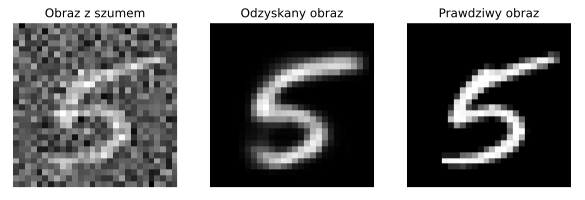
\includegraphics[width=7cm]{denoisingae.pdf}
			\caption{Rekonstrukcja obrazu przy pomocy autoenkodera}
			\label{fig:rekonstrukcja}
		\end{figure}
		\vspace{-0.5cm}
		Zaletą używania autoenkoderów w celu redukcji wymiarów w przeciwieństwie do metody analizy składowych głównych (PCA) jest ich możliwość nauki nieliniowych zależności pomiędzy wymiarami.
	\end{frame}

	\begin{frame}
		\vspace{-1cm}
		\begin{figure}
			\centering\includegraphics[width=10cm]{prawdziwyae.pdf}
		\end{figure}
		\vspace{-0.5cm}
	Odszumianie obrazu zostało wykonane przy pomocy powyższego modelu, składającego się dwóch warstw ukrytych w enkoderze i dekoderze po 120 i 500 neuronów. Funkcje aktywacji to ReLU, poza warstwą kodu, w której jest funkcja liniowa aby nie ograniczać wartości kodu, i w ostatniej sigmoid, ponieważ dane wejściowe są w przedziale 0-1.
	\vspace{-0.5cm}
	\end{frame}

% 6
	\begin{frame}
		\frametitle{Problem generacji danych}
		\subsection{Problem generacji danych}
		Aby wygenerować nowe dane, podobne do tych na których model został wytrenowany, potrzebna jest ściśle określonej dystrybucji według której punkty, reprezentujące skompresowane wejście, są rozłożone. Tradycyjna architektura nie zapewnia tego faktu, ani takich wymagać jak kompletności oraz ciągłości przestrzeni kodu. Przed treningiem nie wiadomo czy losowo wybrany punkt z przestrzeni, będzie generował odpowiednie dane.
	\end{frame}

\begin{frame}  
	\frametitle{Przestrzeń kodu AE}
	\begin{tabular}{cl}  
		\begin{tabular}{c}
			\includegraphics[height=5cm, width=5cm]{aelatentspace.png}
		\end{tabular}
		& \begin{tabular}{l}
			\parbox{0.5\linewidth}{ Obrazek obok przedstawia dwuwymiarową przestrzeń zmiennych ukrytych dla zbioru danych MNIST. Jak widać, nie jest ona kompletna ani ciągła. Wybierany, a następnie odkodowany punkt z miejsca pomiędzy pomarańczowymi a szarymi punktami, nie będzie podobny do obrazów ze zbioru danych.
			}
		\end{tabular}  \\
	\end{tabular}
\end{frame}
		
% 7
	\begin{frame}
		\frametitle{Wariacyjny autoenkoder - wprowadzenie}
		\section{Wariacyjny autoenkoder}
		Wariacyjny autoenkoder rozwiązuje problemy z generacją nowych danych tradycyjnego modelu. Aby model był generacyjny, potrzebujemy ściśle ustalonej dystrybucji, z której losujemy punkty, na podstawie których generujemy dane. W przypadku modelu VAE, jest to wielowymiarowy rozkład normalny, opisywany za pomocą wektorów odchylenia standardowego $\sigma$ oraz średniej $\mu$. Następnie z tych dystrybucji losujemy punkty $z$, które traktujemy jako kod, na podstawie, których rekonstruujemy wejście modelu. Aby wynikiem enkodera były punkty należące do wybranej dystrybucji, trzeba zmodyfikować funkcję straty. Poza błędem rekonstrukcji, obliczamy również dywergencję Kullbacka-Leiblera, która określa rozbieżność pomiędzy dwora rozkładami prawdopodobieństwa. 
	\end{frame}

\begin{frame}  
	\frametitle{Przestrzeń kodu VAE}
	\begin{tabular}{cl}  
		\begin{tabular}{c}
			\includegraphics[height=5cm, width=5cm]{vaelatentspace.png}
		\end{tabular}
		& \begin{tabular}{l}
			\parbox{0.5\linewidth}{Rysunek przestawia dwuwymiarową przestrzeń zmiennych ukrytych dla zbioru MNIST. Jest to przestrzeń wygenerowana przy pomocy modelu VAE, dlatego, jak widać, jest ona dwuwymiarowym rozkładem normalnym. Tym razem możemy wybrać z niej losowy punkt i mieć pewność, że zostanie on poprawnie odkodowany.
			}
		\end{tabular}  \\
	\end{tabular}
\end{frame}

	\begin{frame}
		\frametitle{Architektura wariacyjnego autoenkodera}
		\begin{figure}
			\centering\includegraphics[width=10cm]{tikzvae.pdf}
			% prawdziwa architektura
		\end{figure}
	\end{frame}

	\begin{frame}
		\subsection{Generacja nowych danych}
		\frametitle{Generacja nowych danych}
		Posiadając enkoder, który generuje kod należący co ściśle określonej dystrybucji, można wybierając z niej losowe punkty generować dane. 
		
		\begin{figure}
			\centering\includegraphics{vaegeneracja.png} 
			\caption{Po lewej stronie są dane ze zbioru, a po prawej wygenerowane}
		\end{figure}
	
	Powyższy przykład przedstawia generację na podstawię zbioru danych MNIST.
		
	\end{frame}

	\begin{frame}
		\vspace{-1cm}
		\begin{figure}
			\centering\includegraphics[width=12cm]{prawdziwyvae.pdf}
		\end{figure}
			Cos tutaj bedzie
	\end{frame}

	\begin{frame}
		\begin{center}
			\huge Dziękuje za uwagę!
		\end{center}
	\end{frame}
\end{document}